%%%%%%%%%%%%%%%%%%%%%%%%%%%%%%%%%%%%%%%%%%%%%%%%%%%%%%%%%%%%%%%%%%%%
% Plantilla para proyecto EI-4419: Analisis y Control de Sistemas Lineales
%%%%%%%%%%%%%%%%%%%%%%%%%%%%%%%%%%%%%%%%%%%%%%%%%%%%%%%%%%%%%%%%%%%%

\documentclass[journal]{IEEEtran}

\usepackage{instructivo}
\usepackage{csquotes}
\graphicspath{{./}{informe02/}{informe02/fig/}}

\usepackage[natbib=true,style=trad-unsrt,backend=biber]{biblatex}
\addbibresource{informe02/literatura.bib}

\usepackage{amsmath}
\usepackage{amssymb}
\usepackage{siunitx}
\usepackage{graphicx}
\usepackage{float}
\usepackage{pgfplots}
\pgfplotsset{compat=1.18} % O la versión más reciente disponible en Overleaf
\hyphenation{op-tical net-works semi-conduc-tor}
\hbadness=10000
\vbadness=10000
\hfuzz=1000pt
\vfuzz=1000pt

\title{Modelado y Simulación de un Sistema Electromecánico de Parlantes Acoplados}


\author{~Angulo Vasquez Sebastian~,~Campos Uribe Tomas~
        y~Daniel Montero Vargas.}



% The paper headers
\markboth{EL4419 Análisis y control de sistemas lineales, IS2026}%
{EL4419 Análisis y control de sistemas lineales}

\begin{document}

% make the title area
\maketitle
\begin{abstract}
El presente documento presenta el modelado matemático, la simulación y el diseño de un sistema de control realimentado para un conjunto electromecánico de dos parlantes acoplados. El sistema interconecta el dominio eléctrico y el mecánico mediante transductores bobina-imán idénticos, donde la interacción mutua entre los conos se modela como un acoplamiento viscoso neumático dependiente de la velocidad. Tomando como punto de partida las deficiencias transitorias identificadas en la caracterización de lazo abierto donde la distribución asimétrica de la corriente de excitación (70\% y 30\%) provoca un desfase crítico en el movimiento de los conos, se evalúa inicialmente el desempeño del sistema bajo control proporcional puro ($K_p$). Ante las limitaciones inherentes de la ganancia constante para mitigar las oscilaciones resonantes sin inducir sobreimpulsos severos, se propone e implementa un compensador de adelanto de fase (*lead compensator*) sintonizado analíticamente mediante el Lugar Geométrico de las Raíces. El objetivo de diseño se centra en la reducción drástica del tiempo de asentamiento del error de posición diferencial ($e = x_1 - x_2$) entre ambas membranas acelerando el transitorio sin inducir sobreimpulsos críticos ni oscilaciones resonantes secundarias. Las validaciones se realizan mediante simulaciones numéricas y físicas en las plataformas Simulink y Simscape, demostrando una alta convergencia analítica y una reducción drástica en el tiempo de igualación del movimiento de los conos.





\end{abstract}

% Se sugiere no más de cuatro palabras o frases cortas en orden alfabético, separadas por comas, que representen su reporte
\begin{IEEEkeywords}
Acople, amortiguamiento, rigidez, factor electromecánico.
\end{IEEEkeywords}


%%%%%%%%%%%%%%%%%%%%%%%%%%%%%%%%%%%%%%%%%%%%%%%%%%%%%%%%%%%%%%%%%%%%%%%%%%%%%%%%%%%%%%%%%%%%%%
%%%%%%%%%%%%%%%%%%%%%%%%%%%%%%%%%%%%%%%%%%%%%%%%%%%%%%%%%%%%%%%%%%%%%%%%%%%%%%%%%%%%%%%%%%%%%%
\section{Introducción}

\IEEEPARstart{E}{l} análisis y diseño de sistemas de control lineal aplicados a transductores electrodinámicos representa un área de gran interés en la ingeniería moderna, dada la necesidad de acoplar dinámicas multi-dominio de forma precisa. En arreglos de altavoces adyacentes o integrados en cavidades acústicas compartidas, el movimiento físico de una membrana perturba las condiciones de presión del entorno, induciendo acoplamientos neumáticos y mecánicos mutuos. Este fenómeno altera el comportamiento transitorio y degrada la linealidad de la onda acústica resultante cuando los dispositivos operan bajo condiciones asimétricas de excitación. El presente reporte aborda formalmente esta problemática mediante el modelado analítico y la sintonización de una estrategia de control en lazo cerrado para garantizar el comportamiento uniforme del sistema.

%%%%%%%%%%%%%%%%%%%%%%%%%%%%%%%%%%%%%%%%%%%%%%%%%%%%%%%%%%%%%%%%%%%%%%%%%%%%%%%%%%%%%%%%%%%%%%
%%%%%%%%%%%%%%%%%%%%%%%%%%%%%%%%%%%%%%%%%%%%%%%%%%%%%%%%%%%%%%%%%%%%%%%%%%%%%%%%%%%%%%%%%%%%%%

\subsection{Descripción del Problema y Objetivos}
En aplicaciones prácticas de amplificación y mejora de calidad de audio, se requiere que múltiples parlantes operen sincronizados en fase y amplitud para maximizar la presión sonora total (SPL) y preservar la fidelidad del sonido. Sin embargo, en el escenario planteado, el sistema experimenta una distribución asimétrica en sus fuentes de alimentación, donde el Parlante 1 recibe el 70\% de la corriente de entrada y el Parlante 2 únicamente el 30\%. Esta disparidad eléctrica genera un severo desbalance transitorio en el movimiento de las membranas, lo cual produce fenómenos acústicos destructivos como la cancelación de fase y degradación de la fidelidad acústica.

Ante esta situación, el objetivo primordial consiste en diseñar, simular e implementar un sistema de control realimentado que logre minimizar de forma eficaz el error de velocidad diferencial ($e = V_1 - V_2$) entre ambos conos. Específicamente, se busca reducir de manera drástica el tiempo de asentamiento ($T_s$) en que la membrana del parlante rezagado iguala el desplazamiento del parlante principal, asegurando un transitorio suave y libre de sobreimpulsos críticos que pongan en riesgo la integridad física de los componentes electroacústicos.

%%%%%%%%%%%%%%%%%%%%%%%%%%%%%%%%%%%%%%%%%%%%%%%%%%%%%%%%%%%%%%%%%%%%

\subsection{Descripción del Sistema y Estrategia de Solución}

\begin{figure}[!ht]
\centering
\includegraphics[width=3.0in]{fig/fotoparlante.png}
\caption{Representacion fisica parlante\linebreak}
\end{figure}



Físicamente, el arreglo está constituido por dos altavoces idénticos de bobina móvil colocados en una misma estructura. Cada dispositivo transforma energía eléctrica en trabajo mecánico a través de una bobina inmersa en un campo magnético permanente, cuya interacción queda descrita mecánicamente por un sistema de segundo orden amortiguado (masa, suspensión elástica y fricción). El acoplamiento mutuo entre ambos conos ($\alpha$) se modela como una fuerza disipativa directamente dependiente de la velocidad relativa del medio circundante. 


Para solucionar el desfase mecánico provocado por la asimetría eléctrica, se evalúa inicialmente un lazo de control proporcional puro ($K_p$). No obstante, el análisis dinámico demuestra que el incremento de la ganancia constante no logra resolver la problemática de velocidad sin excitar la resonancia natural del sistema, evocando oscilaciones sostenidas inaceptables. Para mitigar esta deficiencia técnica, se propone la incorporación de un compensador de adelanto de fase (\textit{lead compensator}) sintonizado mediante el Lugar Geométrico de las Raíces (LGR). Esta estructura introduce un cero real que añade un efecto anticipatorio al sistema de control.Esto proporciona un amortiguamiento activo idóneo para obligar a que ambos conos converjan simétricamente de manera casi instantánea.

\subsection{Parámetros del Sistema y Significado Físico}
Para validar las respuestas analíticas y estructurales del modelo acoplado, se emplean parámetros estándar basados en las constantes físicas de Thiele-Small para transductores electrodinámicos de baja señal. Las variables del arreglo se detallan a continuación:

\begin{itemize}
    \item \textbf{Masa Efectiva ($M$):} Representa la masa total del conjunto móvil, el cual incluye el cono de la membrana, el soporte y la bobina de voz de cobre. Su valor determina la inercia del sistema frente a cambios de fuerza.
    
    \item \textbf{Resistencia Mecánica ($R$):} Modela las pérdidas por fricción interna de la suspensión y las pérdidas viscosas iniciales del aire. Actúa como el amortiguador propio del transductor.

    \item \textbf{Rigidez de la Suspensión ($K$):} Define la fuerza restauradora elástica provista de manera combinada por la araña (\textit{spider}) y la suspensión exterior del cono. Determina la tendencia del parlante a retornar a su posición de equilibrio.
    
    \item \textbf{Factor de Fuerza ($Bl$):} Representa el producto de la densidad de flujo magnético del imán ($B$) por la longitud total del conductor de la bobina ($l$). Establece la constante de transformación entre corriente y fuerza, así como de velocidad a fuerza electromotriz inversa.
    
    \item \textbf{Factor de Acoplamiento Mutuo ($\alpha$):} Modela la interacción aerodinámica y de presión entre ambas membranas dentro de la cavidad. Traduce la velocidad de un cono en una fuerza reactiva instantánea sobre el cono adyacente.
\end{itemize}

\subsection{Componentes y Dominios Físicos}
El modelo integra dos dominios físicos principales:
\begin{itemize}
    \item \textbf{Dominio Eléctrico:} Definido por las corrientes de entrada $i_1(t)$ e $i_2(t)$ que actúan sobre las bobinas de voz.
    
    \item \textbf{Dominio Mecánico:} Representado por un sistema de masa-resorte-amortiguador que modela el desplazamiento $x(t)$ y la velocidad $v(t)$ de los conos.
\end{itemize}

\subsection{Origen de las Ecuaciones de Movimiento y Justificación Física}
El origen de las ecuaciones del presente sistema se fundamentan por la segunda ley de Newton ($\sum F = M \cdot a$). Al aislar cada cono de manera independiente mediante un análisis de cuerpo libre, se identifican las fuerzas activas y reactivas que actúan sobre la masa móvil en el eje del desplazamiento unidimensional:

Para el Parlante 1, la fuerza que impulsora del mismo proviene de la ley de Lorentz, expresada como el producto $Bl \cdot i_1$. En oposición al movimiento de la membrana, surgen las fuerzas de restauración elástica del resorte ($-K \cdot x_1$) y la oposición viscosa del amortiguador propio ($-R \cdot \dot{x}_1$). De forma crucial, el acoplamiento introduce una fuerza colineal inducida por el movimiento del segundo parlante, la cual es proporcional a su velocidad ($+\alpha \cdot \dot{x}_2$). Al plantear el balance dinámico se obtiene:
\begin{equation}
    M \ddot{x}_1 = Bl \cdot i_1 - K \cdot x_1 - R \cdot \dot{x}_1 + \alpha \cdot \dot{x}_2
\end{equation}
Reordenando los términos reactivos al miembro izquierdo de la ecuación para dar forma al modelo dinámico estándar, generando la ecuación fundamental del sistema:
\begin{equation}
    M \ddot{x}_1 + R \dot{x}_1 + K x_1 = Bl \cdot i_1 + \alpha \dot{x}_2
\end{equation}

Al realizar el análisis de cuerpo libre sobre la masa del Parlante 2 se puede notar que movimiento responde a la fuerza eléctrica de su propia bobina ($Bl \cdot i_2$) y al arrastre neumático proveniente de la velocidad del primer cono ($+\alpha \cdot \dot{x}_1$), lo que resulta en:

\begin{equation}
    M \ddot{x}_2 + R \dot{x}_2 + K x_2 = Bl \cdot i_2 + \alpha \dot{x}_1
\end{equation}

\section{Modelo matemático}
Para el desarrollo del modelo se baso las ecuaciones en la segunda ley de Newton.

\begin{equation}
M\ddot{x} + R\dot{x} + Kx = F + \alpha\ 
\end{equation}

Está ecuación se duplica ya que una representa el parlante 1 y la otra ecuación el parlante 2. 
\begin{equation}
    M\ddot{x}_1 + R\dot{x}_1 + kx_1 = Bl i_1 + \alpha \dot{x}_2
\end{equation}

\begin{equation}
    M\ddot{x}_2 + R\dot{x}_2 + kx_2 = Bl i_2 + \alpha \dot{x}_1
\end{equation}

De estos dos sistemas se definen las siguientes variables:

\begin{itemize}
\item $x_1, x_2$: desplazamientos.
\item $\dot{x}_1, \dot{x}_2$: velocidades.
\item $\ddot{x}_1, \ddot{x}_2$: aceleraciones.
\item $i_1, i_2$: corrientes de entrada.
\end{itemize}

\subsection{Función de transferencia}
Como primer paso se realiza la transformada de Laplace de la ecuaciones.

\begin{equation*}
    Ms^2X_1(s) + RsX_1(s) + kX_1(s) = Bl I_1(s) + \alpha {X}_2(s)  
\end{equation*}


\begin{equation*}
   Ms^2{X}_2(s) + Rs{X}_2(s) + kX_2(s) = Bl I_2(s) + \alpha {X}_1(s)
\end{equation*}


Como segundo paso se agrupan las expresiones comunes de los sistemas para simplificar las ecuaciones.


\begin{equation*}
    D(s)= Ms^2 + Rs + k    
\end{equation*}

Primera ecuación.
\begin{equation*}
    D(s){X}_1(s)= Bl I_1(s) + \alpha {X}_2(s)
\end{equation*}

Segunda ecuación.
\begin{equation*}
    D(s)X_2(s) = Bl I_2(s) + \alpha {X}_1(s)
\end{equation*}

Como tercer paso nos encontramos que ambas ecuaciones dependen tanto de $X_1$ como de $X_2$, para obtener uno de estos dos valores sin depender del otro empleamos la regla de Crammer.

\begin{equation*}
\begin{bmatrix} D(s) & -{\alpha}s \\ -{\alpha}s & D(s) \end{bmatrix} + 
\begin{bmatrix} X_1  \\ X_2  \end{bmatrix} = 
\begin{bmatrix} I_1*Bl \\ I_2*Bl \end{bmatrix}
\end{equation*}

Calculamos el valor de la matriz original.

\begin{equation*}
  \Delta= D(s)^2- (\alpha s)^2
\end{equation*}

Seguidamente se calcula los determinantes de $X_1$ y $X_2$

\begin{equation*}
  \Delta_{X_1}= Bl*I_1*D(s)+ \alpha*s*Bl*I_2
\end{equation*}

\begin{equation*}
  \Delta_{X_2}= Bl*I_2*D(s)+ \alpha*s*Bl*I_1
\end{equation*}

De este modo las ecuaciones de los desplazamientos de los conos de los dos parlantes se determinará del siguiente modo:

\begin{equation*}
  X_1= \frac{Bl*I_1*D(s)+ \alpha*s*Bl*I_2}{D(s)^2- (\alpha s)^2} 
\end{equation*}

\begin{equation*}
  X_2= \frac{Bl*I_2*D(s)- \alpha*s*Bl*I_1}{D(s)^2- (\alpha s)^2} 
\end{equation*}


Se debe de recordar que lo que se precisa obtener es la velocidad  con la que se desplaza el cono, por lo que se debe de realizar la siguiente sustitución en ambas ecuaciones $V=X(s)*s$.
Además la corriente que alimenta a los parlantes es una misma, solo que el primer parlante consume el 70\% de la corriente ($I_1$), mientras que el parlante 2 consume el 30\% restante ($I_2$).


\begin{equation*}
  V_1= \frac{Bl*s*(0.7*I(S)*D(s)+ 0.3*\alpha*s*I(s))}{D(s)^2- (\alpha s)^2} 
\end{equation*}

\begin{equation*}
  V_2= \frac{Bl*s*(0.3*I(s)*D(s)- \alpha*s*I(s)*0.7)}{D(s)^2- (\alpha s)^2} 
\end{equation*}

Por último se sustituye la equivalencia de D(s) y se reemplazan los valores de las constantes para obtener el valor de las funciones de transferencia.

Cálculo del denominador.

\begin{equation*}
\begin{aligned}
  \Delta ={}& 7.84*10^{-4}s^{4}+0.056s^3+80.97s^2 \\
  &+2857.14s+2040812.245
\end{aligned}
\end{equation*}

Función de transferencia del parlante 1.
\begin{equation*}
  \frac{V_1}{I}= \frac{0.196s^3+7.9s^2+9999.99s}{\Delta}
\end{equation*}
Función de transferencia del parlante 2.
\begin{equation*}
  \frac{V_2}{I}= \frac{0.0854s^3+5.1s^2+4285.71s}{\Delta} 
\end{equation*}



\subsection{Interpretación de las funciones de transferencia}

Ambos parlantes presentan el mismo denominador común en sus funciones de transferencia 

\begin{equation}
\Delta(s) = D(s)^2 - (\alpha s)^2
\end{equation}

Este término es relevante debido a que permite interpretar directamente el efecto del acoplamiento entre parlantes. En ausencia de acoplamiento ($\alpha =0$), el sistema se encuentra en desacople y su comportamiento consistiría de dos sistemas totalmente independientes de segundo orden.


La parte del término donde se presenta $(\alpha s)^2$ introduce la dinámica que modifica la posición de los polos del sistema, de forma que su estabilidad y respuesta temporal se ve afectada. Esto implica que ya el modelado como dos sistemas independientes no es posible, y se debe tomar como uno solo de cuarto orden acoplado.

Por otra parte, los numeradores de cada funcion de transferencia determinan los ceros. Para este modelo los ceros dependen del comportamiento de la corriente entre ambos parlantes y del acoplamiento mecánico. Es por esto que las funciones comparten los polos, apesar de que sus respuestas temporales si son diferentes. 

A grandes rasgos estos ceros modifican la respuesta transitoria, la amplitud relativa y la manera en que cada parlante reacciona ante una misma entrada. En base a esto es claro que el parlante con mayor corriente directamente presenta más excitación, mientras que el otro parlante responde tanto por la corriente aplicada como por la influencia del acople.

\subsection{Suposiciones del modelo}

% Listar las suposiciones utilizadas para simplificar el modelo.

Para el desarrollo del modelo matemático se establecieron las siguientes suposiciones:

\begin{itemize}
    \item Los parlantes se consideran idénticos, por lo que sus parámetros físicos son iguales.
    
    \item El comportamiento del sistema es lineal, asumiendo pequeñas oscilaciones alrededor del punto de equilibrio.
    
    \item La fuerza electromagnética es proporcional a la corriente de entrada, modelada mediante la constante $Bl$.
    
    \item El acoplamiento entre parlantes depende únicamente de la velocidad relativa, representado por el término $\alpha \dot{x}$.
    
    \item No se consideran efectos no lineales como saturación magnética, histéresis o deformaciones estructurales.
    
    \item Se asume que las condiciones iniciales del sistema son cero.
\end{itemize}

\section{Diagrama Funcional}

% Insertar y explicar el diagrama funcional del sistema.

%\begin{figure}[H]
 %   \centering
  %  \includegraphics[width=0.45\textwidth]{fig/diagrama_funcional.pdf}
   % \caption{Diagrama funcional del sistema seleccionado.}
    %\ {fig:diagrama_funcional}
%\end{figure}

\begin{figure}[!t]
\centering
\shorthandoff{>}
\resizebox{\columnwidth}{!}{
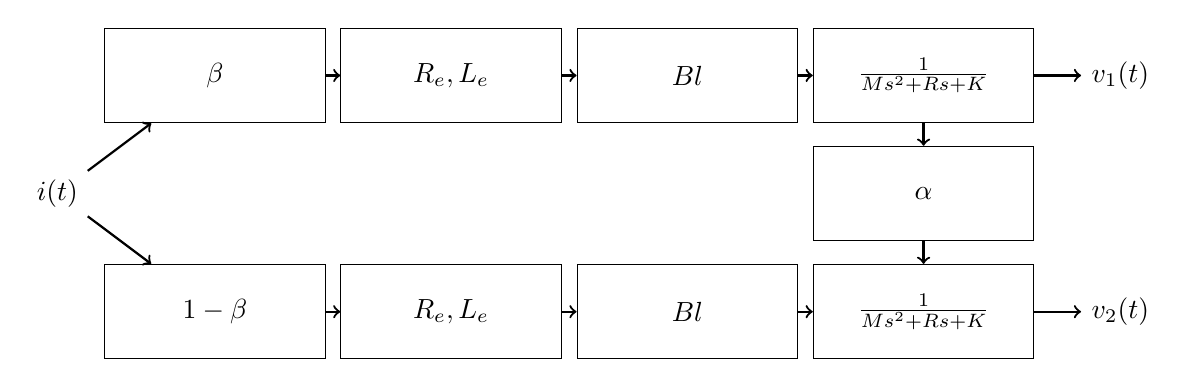
\begin{tikzpicture}[
    block/.style={rectangle, draw, minimum width=2.8cm, minimum height=1.2cm},
    arrow/.style={->, thick}
]
% Entrada
\node (input) at (0,0) {$i(t)$};

% Beta bloques
\node[block] (beta1) at (2,1.5) {$\beta$};
\node[block] (elec1) at (5,1.5) {$R_e, L_e$};
\node[block] (bl1)   at (8,1.5) {$Bl$};
\node[block] (mech1) at (11,1.5) {$\frac{1}{Ms^2 + Rs + K}$};
\node at (13.5,1.5) {$v_1(t)$};

% 1 - beta bloques
\node[block] (beta2) at (2,-1.5) {$1 - \beta$};
\node[block] (elec2) at (5,-1.5) {$R_e, L_e$};
\node[block] (bl2)   at (8,-1.5) {$Bl$};
\node[block] (mech2) at (11,-1.5) {$\frac{1}{Ms^2 + Rs + K}$};
\node at (13.5,-1.5) {$v_2(t)$};

\node[block] (alpha) at (11,0) {$\alpha$};

% i
\draw[arrow] (input) -- (beta1);
\draw[arrow] (input) -- (beta2);

% Beta flechas
\draw[arrow] (beta1) -- (elec1);
\draw[arrow] (elec1) -- (bl1);
\draw[arrow] (bl1) -- (mech1);
\draw[arrow] (mech1) -- (13,1.5);

% 1 - Beta flechas
\draw[arrow] (beta2) -- (elec2);
\draw[arrow] (elec2) -- (bl2);
\draw[arrow] (bl2) -- (mech2);
\draw[arrow] (mech2) -- (13,-1.5);

% Alfa glechas
\draw[arrow] (mech1) -- (alpha);
\draw[arrow] (alpha) -- (mech2);

\end{tikzpicture}
}
\shorthandon{>}
\caption{Modelo de parlantes con distribución de corriente}
\end{figure}



%%%%%%%%%%%%%%%%%%%%%%%%%%%%%%%%%%%%%%%%%%%%%%%%%%%%%%%%%%%%%%%%%%

% Presentar entradas, salidas, variables internas y parámetros físicos.

\begin{table}[H]
\centering
\caption{Parámetros y variables utilizados en el modelo}
\scriptsize
\begin{tabular}{|c|c|}
\hline
\textbf{Parámetro / variable} & \textbf{Valor / definición} \
\hline
$M$ & $0.028\ \mathrm{kg}$ \
\hline
$R$ & $1\ \mathrm{N,s/m}$ \
\hline
$Bl$ & $10\ \mathrm{N/A}$ \
\hline
$C_{ms}$ & $0.0007\ \mathrm{m/N}$ \
\hline
$K$ & $\frac{1}{C_{ms}}=1428.57\ \mathrm{N/m}$ \
\hline
$\alpha$ & $0.03$ \
\hline
$\beta$ & $0.7$ \
\hline
$1-\beta$ & $0.3$ \
\hline
$i(t)$ & Corriente total de entrada \
\hline
$i_1(t)$ & $\beta i(t)$ \
\hline
$i_2(t)$ & $(1-\beta)i(t)$ \
\hline
$x_1(t)$ & Desplazamiento del parlante 1 \
\hline
$x_2(t)$ & Desplazamiento del parlante 2 \
\hline
$v_1(t)$ & $\dot{x}*1(t)$ \
\hline
$v_2(t)$ & $\dot{x}*2(t)$ \
\hline
$x(t)$ & $\begin{bmatrix}x_1 & v_1 & x_2 & v_2\end{bmatrix}^{T}$ \
\hline
$y(t)$ & $\begin{bmatrix}v_1 & v_2\end{bmatrix}^{T}$ \
\hline
$u(t)$ & Señal de control aplicada a la planta \
\hline
$r(t)$ & Referencia de velocidad \
\hline
$e(t)$ & $r(t)-v_1(t)$ \
\hline
$G_v(s)$ & $\frac{V_1(s)}{I(s)}$ \
\hline
$K_c$ & $0.4755$ \
\hline
$z$ & $30$ \
\hline
$p$ & $124$ \
\hline
$C(s)$ & $0.4755\frac{s+30}{s+124}$ \
\hline
$\zeta*{\mathrm{actual}}$ & $0.077$ \
\hline
$\zeta_d$ & $0.30$ \
\hline
$s_d$ & $-60\pm j190.8$ \
\hline
$A*{\mathrm{seno}}$ & $0.01\ \mathrm{m/s}$ \
\hline
$f_{\mathrm{seno}}$ & $5\ \mathrm{Hz}$ \
\hline
$\omega_{\mathrm{seno}}$ & $2\pi f_{\mathrm{seno}}=31.42\ \mathrm{rad/s}$ \
\hline
\end{tabular}
\end{table}


\subsection{Ecuaciones físicas del sistema}

% Derivar las ecuaciones desde leyes físicas.

\subsection{Modelo en espacio de estados}

% Definir variables de estado.
% Derivar matrices A, B, C y D directamente desde el modelo físico.

\begin{equation}
\dot{x}(t) = Ax(t) + Bu(t)
\end{equation}

\begin{equation}
y(t) = Cx(t) + Du(t)
\end{equation}

\subsection{Espacio de estados}
Nuevamente se emplean las ecuaciones 2.2 y 2.3, despejando la aceleración del sistema.

\begin{equation*}
    \ddot{x}_1 = -\frac{R\dot{x}_1}{M}  -\frac{kx_1}{M} + \frac{0.7*Bl}{M} +  \frac{\alpha \dot{x}_2}{M}
\end{equation*}

\begin{equation*}
   \ddot{x}_1 = -\frac{R\dot{x}_2}{M}  -\frac{kx_2}{M} + \frac{0.3*Bl}{M} +  \frac{\alpha \dot{x}_1}{M}
\end{equation*}

Seguidamente se define el vector de estados y se deriva.

Vector de estados.
\begin{equation*}
x=\begin{bmatrix} x_1  \\  v_1  \\ x_2  \\ v_2 \end{bmatrix} 
\end{equation*}

Vector derivado.
\begin{equation*}
\dot{x}=\begin{bmatrix} \dot{x_1}  \\  \dot{v_1}  \\ \dot{x_2}  \\ \dot{v_2} \end{bmatrix} 
\end{equation*}

Vector de respuestas.
\begin{equation*}
y=\begin{bmatrix} v_1 \\ v_2 \end{bmatrix} 
\end{equation*}


Como tercer paso se acomodan las ecuaciones en sus respectivas matrices.


\begin{equation*}
A=\begin{bmatrix} 0 & 1 & 0 & 0 \\ -\frac{k}{M} & -\frac{R}{M}& 0 & \frac{\alpha}{M} \\ 0 & 0 & 0 & 1 \\ 0 & \frac{\alpha}{M} & -\frac{k}{M}& -\frac{R}{M}  \end{bmatrix}
\end{equation*}

\begin{equation*}
B=\begin{bmatrix} 0  \\  0.7\frac{Bl}{M} \\ 0  \\ 0.3\frac{Bl}{M}  \end{bmatrix}
\end{equation*}

\begin{equation*}
C=\begin{bmatrix} 0 & 1 & 0 & 0 \\ 0 & 0 & 0 & 1 \\ \end{bmatrix}
\end{equation*}

\begin{equation*}
D=\begin{bmatrix} 0 & 0 \\ 0 & 0 \\ \end{bmatrix}
\end{equation*}


Por ultimo se reemplazan los valores numéricos en las matrices correspondientes.

\begin{equation*}
A=\begin{bmatrix} 0 & 1 & 0 & 0 \\ -51020.36 & -35.71& 0 & 10.71 \\ 0 & 0 & 0 & 1 \\ 0 & 10.71 & -51020.36 & -35.71 \end{bmatrix}
\end{equation*}

\begin{equation*}
B=\begin{bmatrix} 0  \\  250 \\ 0  \\ 107.14  \end{bmatrix}
\end{equation*}
%%%%%%%%%%%%%%%%%%%%%%%%%%%%%%%%%%%%%%%%%%%%%%%%%%%%%%%%%%%%%%%%%%

%%%%%%%%%%%%%%%%%%%%%%%%%%%%%%%%%%%%%%%%%%%%%%%%%%%%%%%%%%%%%%%%%%

%%%%%%%%%%%%%%%%%%%%%%%%%%%%%%%%%%%%%%%%%%%%%%%%%%%%%%%%%%%%%%%%%%%%

\section{Diseño del compensador en adelanto}

Una vez obtenido y validado el modelo dinámico de los parlantes acoplados, se procedió a diseñar un compensador para mejorar la respuesta transitoria del sistema. Para esta etapa se seleccionó como variable controlada la velocidad del primer parlante, $v_1(t)$, debido a que el acoplamiento entre ambos parlantes fue modelado mediante términos dependientes de velocidad. La velocidad del segundo parlante, $v_2(t)$, se mantiene como variable observada para analizar el efecto del acoplamiento sobre el sistema completo.

La planta utilizada para el diseño corresponde a la relación entre la corriente de entrada y la velocidad del primer parlante:

\begin{equation}
G_v(s)=\frac{V_1(s)}{I(s)}
\end{equation}

A partir de los parámetros definidos para el sistema, la función de transferencia de velocidad del primer parlante queda dada por:

\begin{equation}
G_v(s)=
\frac{0.196s^3+7.09s^2+10000s}
{0.000784s^4+0.056s^3+80.9991s^2+2857.14s+2040816.33}
\end{equation}

El numerador de esta función de transferencia presenta un cero en el origen, lo cual indica que la velocidad tiende a cero ante una entrada constante. Esto es físicamente coherente, ya que una corriente constante produce una fuerza constante que desplaza la membrana hasta alcanzar una nueva posición de equilibrio; una vez alcanzado dicho equilibrio, la velocidad desaparece.

Los ceros de la planta son aproximadamente:

\begin{equation}
s=0
\end{equation}

\begin{equation}
s \approx -18.09 \pm j225.15
\end{equation}

mientras que los polos son:

\begin{equation}
s \approx -18.39 \pm j225.13
\end{equation}

\begin{equation}
s \approx -17.32 \pm j225.21
\end{equation}

Todos los polos se encuentran en el semiplano izquierdo, por lo que la planta sin compensar es estable. Sin embargo, los polos dominantes se encuentran cercanos al eje imaginario, lo cual produce una respuesta oscilatoria con bajo amortiguamiento.

Para los polos dominantes:

\begin{equation}
s \approx -17.32 \pm j225.21
\end{equation}

el factor de amortiguamiento se calcula como:

\begin{equation}
\zeta =
\frac{\sigma}{\sqrt{\sigma^2+\omega_d^2}}
\end{equation}

donde $\sigma=17.32$ y $\omega_d=225.21$. Por tanto:

\begin{equation}
\zeta =
\frac{17.32}{\sqrt{17.32^2+225.21^2}}
\approx 0.077
\end{equation}

Este valor confirma que la planta posee un bajo amortiguamiento. Por esta razón, el objetivo del compensador no es estabilizar el sistema, sino mejorar su respuesta transitoria, reduciendo la oscilación y acelerando el decaimiento de la velocidad.

Se seleccionó un factor de amortiguamiento deseado de:

\begin{equation}
\zeta_d = 0.30
\end{equation}

y una frecuencia natural de diseño de:

\begin{equation}
\omega_n = 200 \ \text{rad/s}
\end{equation}

Con estos valores, el polo deseado se obtiene mediante:

\begin{equation}
s_d=-\zeta_d\omega_n \pm j\omega_n\sqrt{1-\zeta_d^2}
\end{equation}

Sustituyendo:

\begin{equation}
s_d = -0.30(200) \pm j200\sqrt{1-0.30^2}
\end{equation}

\begin{equation}
s_d \approx -60 \pm j190.8
\end{equation}

Este punto representa una respuesta más amortiguada que la original, ya que la parte real se desplaza desde aproximadamente $-17.32$ hasta $-60$, provocando un decaimiento más rápido del transitorio.

El compensador seleccionado fue un compensador en adelanto, definido como:

\begin{equation}
C(s)=K_c\frac{s+z}{s+p}
\end{equation}

donde $p>z$, de forma que el polo del compensador se ubica más a la izquierda que el cero. Esta configuración permite aportar fase positiva y desplazar el lugar de raíces hacia una región de mayor amortiguamiento.

Para que el punto $s_d$ pertenezca al lugar de raíces del sistema compensado, debe cumplirse la condición de ángulo:

\begin{equation}
\angle C(s_d)G_v(s_d)=(2k+1)180^\circ
\end{equation}

Al evaluar la planta sin compensar en el punto deseado se obtuvo:

\begin{equation}
\angle G_v(s_d) \approx 152.57^\circ
\end{equation}

Por tanto, la fase adicional que debe aportar el compensador es:

\begin{equation}
\phi_c = 180^\circ - 152.57^\circ
\end{equation}

\begin{equation}
\phi_c \approx 27.43^\circ
\end{equation}

Se seleccionó un cero en:

\begin{equation}
z=30
\end{equation}

lo cual corresponde a un cero ubicado en $s=-30$. A partir de la geometría del lugar de raíces, el ángulo desde este cero hacia el punto deseado es:

\begin{equation}
\theta_z=\angle(s_d+30)
\end{equation}

\begin{equation}
\theta_z=\angle(-30+j190.8)\approx 98.94^\circ
\end{equation}

El compensador debe aportar:

\begin{equation}
\theta_z-\theta_p=27.43^\circ
\end{equation}

por lo que:

\begin{equation}
\theta_p=98.94^\circ-27.43^\circ
\end{equation}

\begin{equation}
\theta_p\approx71.51^\circ
\end{equation}

El polo del compensador se ubica en $s=-p$, por lo que:

\begin{equation}
s_d+p=(p-60)+j190.8
\end{equation}

Aplicando la relación trigonométrica:

\begin{equation}
\tan(\theta_p)=\frac{190.8}{p-60}
\end{equation}

se obtiene:

\begin{equation}
p=60+\frac{190.8}{\tan(71.51^\circ)}
\end{equation}

\begin{equation}
p\approx124
\end{equation}

Por tanto, la parte dinámica del compensador queda como:

\begin{equation}
C_0(s)=\frac{s+30}{s+124}
\end{equation}

Luego se aplicó la condición de magnitud:

\begin{equation}
|K_cC_0(s_d)G_v(s_d)|=1
\end{equation}

Despejando la ganancia del compensador:

\begin{equation}
K_c=\frac{1}{|C_0(s_d)||G_v(s_d)|}
\end{equation}

Al evaluar en el punto de diseño se obtuvo:

\begin{equation}
|G_v(s_d)|\approx2.191
\end{equation}

\begin{equation}
|C_0(s_d)|\approx0.960
\end{equation}

Por tanto:

\begin{equation}
K_c=\frac{1}{(2.191)(0.960)}
\end{equation}

\begin{equation}
K_c\approx0.4755
\end{equation}

Finalmente, el compensador diseñado queda dado por:

\begin{equation}
C(s)=0.4755\frac{s+30}{s+124}
\end{equation}

Con este compensador, los polos del sistema en lazo cerrado se ubicaron aproximadamente en:

\begin{equation}
s=-59.96 \pm j190.77
\end{equation}

\begin{equation}
s=-18.08 \pm j225.15
\end{equation}

\begin{equation}
s=-158.22
\end{equation}

El par de polos ubicado cerca de $s=-60\pm j190.8$ confirma que el diseño permitió alcanzar la región dinámica deseada. Aunque aparece otro par de polos más cercano al eje imaginario, este se encuentra prácticamente cancelado por los ceros cercanos de la planta, por lo que su efecto sobre la respuesta temporal es reducido.

\section{Implementación del compensador en Simulink}

El compensador diseñado se implementó en Simulink mediante un bloque de función de transferencia con la forma:

\begin{equation}
C(s)=K_c\frac{s+z}{s+p}
\end{equation}

donde se utilizaron los valores:

\begin{equation}
K_c=0.4755, \quad z=30, \quad p=124
\end{equation}

Por tanto, en el bloque de función de transferencia del compensador se configuró el numerador como:

\begin{equation}
K_c[1 \quad z]
\end{equation}

y el denominador como:

\begin{equation}
[1 \quad p]
\end{equation}

La implementación se realizó en lazo cerrado con realimentación negativa unitaria de la velocidad del primer parlante. La estructura general del sistema compensado se puede describir mediante:

\begin{equation}
e(t)=r(t)-v_1(t)
\end{equation}

\begin{equation}
u(t)=C(s)e(t)
\end{equation}

\begin{equation}
v_1(t)=G_v(s)u(t)
\end{equation}

donde $r(t)$ es la referencia de velocidad, $e(t)$ es la señal de error, $u(t)$ es la señal de control producida por el compensador y $v_1(t)$ es la velocidad del parlante principal.

La salida del compensador $u(t)$ se utilizó como entrada común para la función de transferencia del primer parlante, la función de transferencia del segundo parlante y el modelo en espacio de estados. Sin embargo, la señal de realimentación se tomó únicamente desde $v_1(t)$, ya que esta es la variable controlada. La velocidad $v_2(t)$ se mantuvo como una salida observada para analizar la respuesta del segundo parlante acoplado.

La estructura implementada puede resumirse como:

\begin{equation}
r(t) \rightarrow e(t) \rightarrow C(s) \rightarrow G_v(s) \rightarrow v_1(t)
\end{equation}

con realimentación negativa desde $v_1(t)$ hacia el sumador de entrada.

\begin{figure}[H]
    \centering
    \includegraphics[width=0.48\textwidth]{modelo_simulink_compensado.png}
    \caption{Modelo en Simulink del sistema compensado en velocidad.\linebreak}
    \ {fig:modelo simulink compensado}
\end{figure}

Para facilitar el análisis posterior, se agregaron bloques \textit{To Workspace} en las señales principales del sistema. Las señales exportadas fueron la velocidad del primer parlante $v_1(t)$, la velocidad del segundo parlante $v_2(t)$ y la señal de control $u(t)$. Estas señales fueron posteriormente almacenadas en archivos de resultados para generar las gráficas utilizadas en el análisis.

\section{Simulaciones del sistema compensado}

Con el compensador implementado, se realizaron simulaciones ante dos tipos de entrada: una referencia escalón y una referencia senoidal. La primera permite observar la mejora del transitorio respecto al sistema sin compensar, mientras que la segunda permite evaluar el comportamiento del sistema ante una señal periódica.

\subsection{Respuesta ante entrada escalón}

En la primera simulación se aplicó una entrada tipo escalón al sistema compensado como señal de prueba para evaluar el comportamiento transitorio. El propósito de esta prueba fue observar la reducción de la oscilación y del tiempo de asentamiento en la velocidad del primer parlante.

\begin{figure}[H]
    \centering
    \includegraphics[width=0.48\textwidth]{ScopePrintToFigure.pdf}
    \caption{Respuesta en velocidad del sistema compensado ante una entrada escalón.\linebreak}
    \ {fig:respuesta compensada escalon}
\end{figure}

A partir de la respuesta obtenida se observa que el compensador en adelanto reduce de forma significativa la oscilación inicial de la velocidad. En comparación con el caso sin compensador, la velocidad del primer parlante presenta un transitorio de menor duración y una respuesta más amortiguada.

Es importante señalar que la velocidad tiende nuevamente a cero después del transitorio. Este comportamiento no representa un error del compensador, sino una característica propia de la planta de velocidad, ya que la función de transferencia $G_v(s)$ posee un cero en el origen. Ante una entrada constante, el sistema mecánico alcanza una posición de equilibrio y la velocidad desaparece.

Por tanto, el objetivo del compensador no fue modificar el valor final de la velocidad ante una entrada constante, sino mejorar el comportamiento transitorio del sistema. En este sentido, el compensador permitió disminuir el pico inicial, reducir el número de oscilaciones visibles y aumentar el amortiguamiento efectivo de la respuesta.

La respuesta del segundo parlante presenta una amplitud menor que la del primero, lo cual es coherente con la distribución de corriente definida por el parámetro $\beta=0.7$. Además, debido a que $v_2(t)$ no forma parte directa del lazo de realimentación, su comportamiento se interpreta como una respuesta acoplada del sistema completo.

\subsection{Respuesta ante entrada senoidal}

En la segunda simulación se utilizó una referencia senoidal de velocidad definida como:

\begin{equation}
r(t)=0.01\sin(2\pi 5t)
\end{equation}

Esta entrada permite analizar la respuesta del sistema ante una señal periódica, lo cual resulta relevante debido a que los parlantes normalmente operan bajo excitaciones variables en el tiempo.

\begin{figure}[H]
    \centering
    \includegraphics[width=0.48\textwidth]{respuesta_compensada_senoidal.pdf}
    \caption{Respuesta en velocidad del sistema compensado ante una entrada senoidal.\linebreak}
\end{figure}

La simulación muestra que el sistema compensado mantiene una respuesta estable ante la entrada senoidal. La velocidad del primer parlante presenta una respuesta periódica estable, con la misma naturaleza oscilatoria de la entrada senoidal, aunque con una amplitud menor a la referencia aplicada. Por otro lado, la velocidad del segundo parlante mantiene una amplitud menor, lo cual es coherente con la distribución de corriente y con el hecho de que esta variable no se encuentra directamente en el lazo de realimentación.

La señal de control generada por el compensador modifica la corriente aplicada al sistema con el fin de mejorar el comportamiento de la variable controlada. Aunque el segundo parlante no se realimenta directamente, su respuesta se ve afectada por la misma señal de control y por el acoplamiento mecánico presente en el modelo.

Esta simulación permite verificar que el compensador no solo mejora la respuesta transitoria ante una entrada escalón, sino que también mantiene un comportamiento estable ante una señal variable en el tiempo.

\subsection{Comparación general del sistema compensado}

El sistema sin compensar presentaba polos dominantes con un factor de amortiguamiento aproximado de $\zeta=0.077$, lo que producía una respuesta oscilatoria y poco amortiguada. Con el diseño del compensador en adelanto, se buscó desplazar la dinámica dominante hacia una región asociada a un amortiguamiento deseado de $\zeta_d=0.30$.

Los polos obtenidos para el sistema compensado muestran que la dinámica principal se desplazó hacia valores con una parte real más negativa. Esto implica un decaimiento más rápido de la envolvente temporal y una reducción de las oscilaciones observables en la respuesta.

Por tanto, el compensador diseñado cumple con el objetivo planteado: mejorar el comportamiento transitorio de la velocidad del primer parlante sin comprometer la estabilidad del sistema.

\section{Conclusiones}

% Conclusiones técnicas del modelado, simulación y validación.

La representación en espacio de estados permitió describir la dinámica interna del sistema, mientras que las funciones de transferencia permitieron analizar la relación entrada-salida en el dominio de Laplace. La validación mediante Simulink y Simscape mostró una alta concordancia entre los modelos.

El acoplamiento entre parlantes modifica la dinámica del sistema, ya que introduce interacción entre las velocidades de ambos conos. Además, aunque ambos parlantes comparten los mismos polos, sus ceros son distintos, lo que explica las diferencias en amplitud y forma de la respuesta temporal.

Adicionalmente, es importante recalcar el diseño e implementación del compensador en adelanto para mejorar la respuesta transitoria de la velocidad del primer parlante. A partir del análisis de polos se determinó que el sistema sin compensar era estable, pero presentaba bajo amortiguamiento, con un valor aproximado de \(\zeta=0.077\). Mediante el diseño por lugar de raíces se obtuvo el compensador \(C(s)=0.4755(s+30)/(s+124)\), con el cual se logró desplazar la dinámica principal hacia una región de mayor amortiguamiento. Las simulaciones ante entrada escalón y senoidal mostraron una respuesta estable, con reducción de oscilaciones y menor duración del transitorio.

Finalmente, se verificó que el sistema es estable para los parámetros utilizados, debido a la presencia de amortiguamiento mecánico y a que las respuestas temporales tienden a estabilizarse después del transitorio.

%%%%%%%%%%%%%%%%%%%%%%%%%%%%%%%%%%%%%%%%%%%%%%%%%%%%%%%%%%%%%%%%%%%%
\printbibliography

\end{document}